\documentclass[border=5mm]{standalone}
\usepackage[utf8]{inputenc}
\usepackage{tikz}
\usetikzlibrary{positioning, arrows.meta, shapes.geometric, fit, backgrounds}

\begin{document}
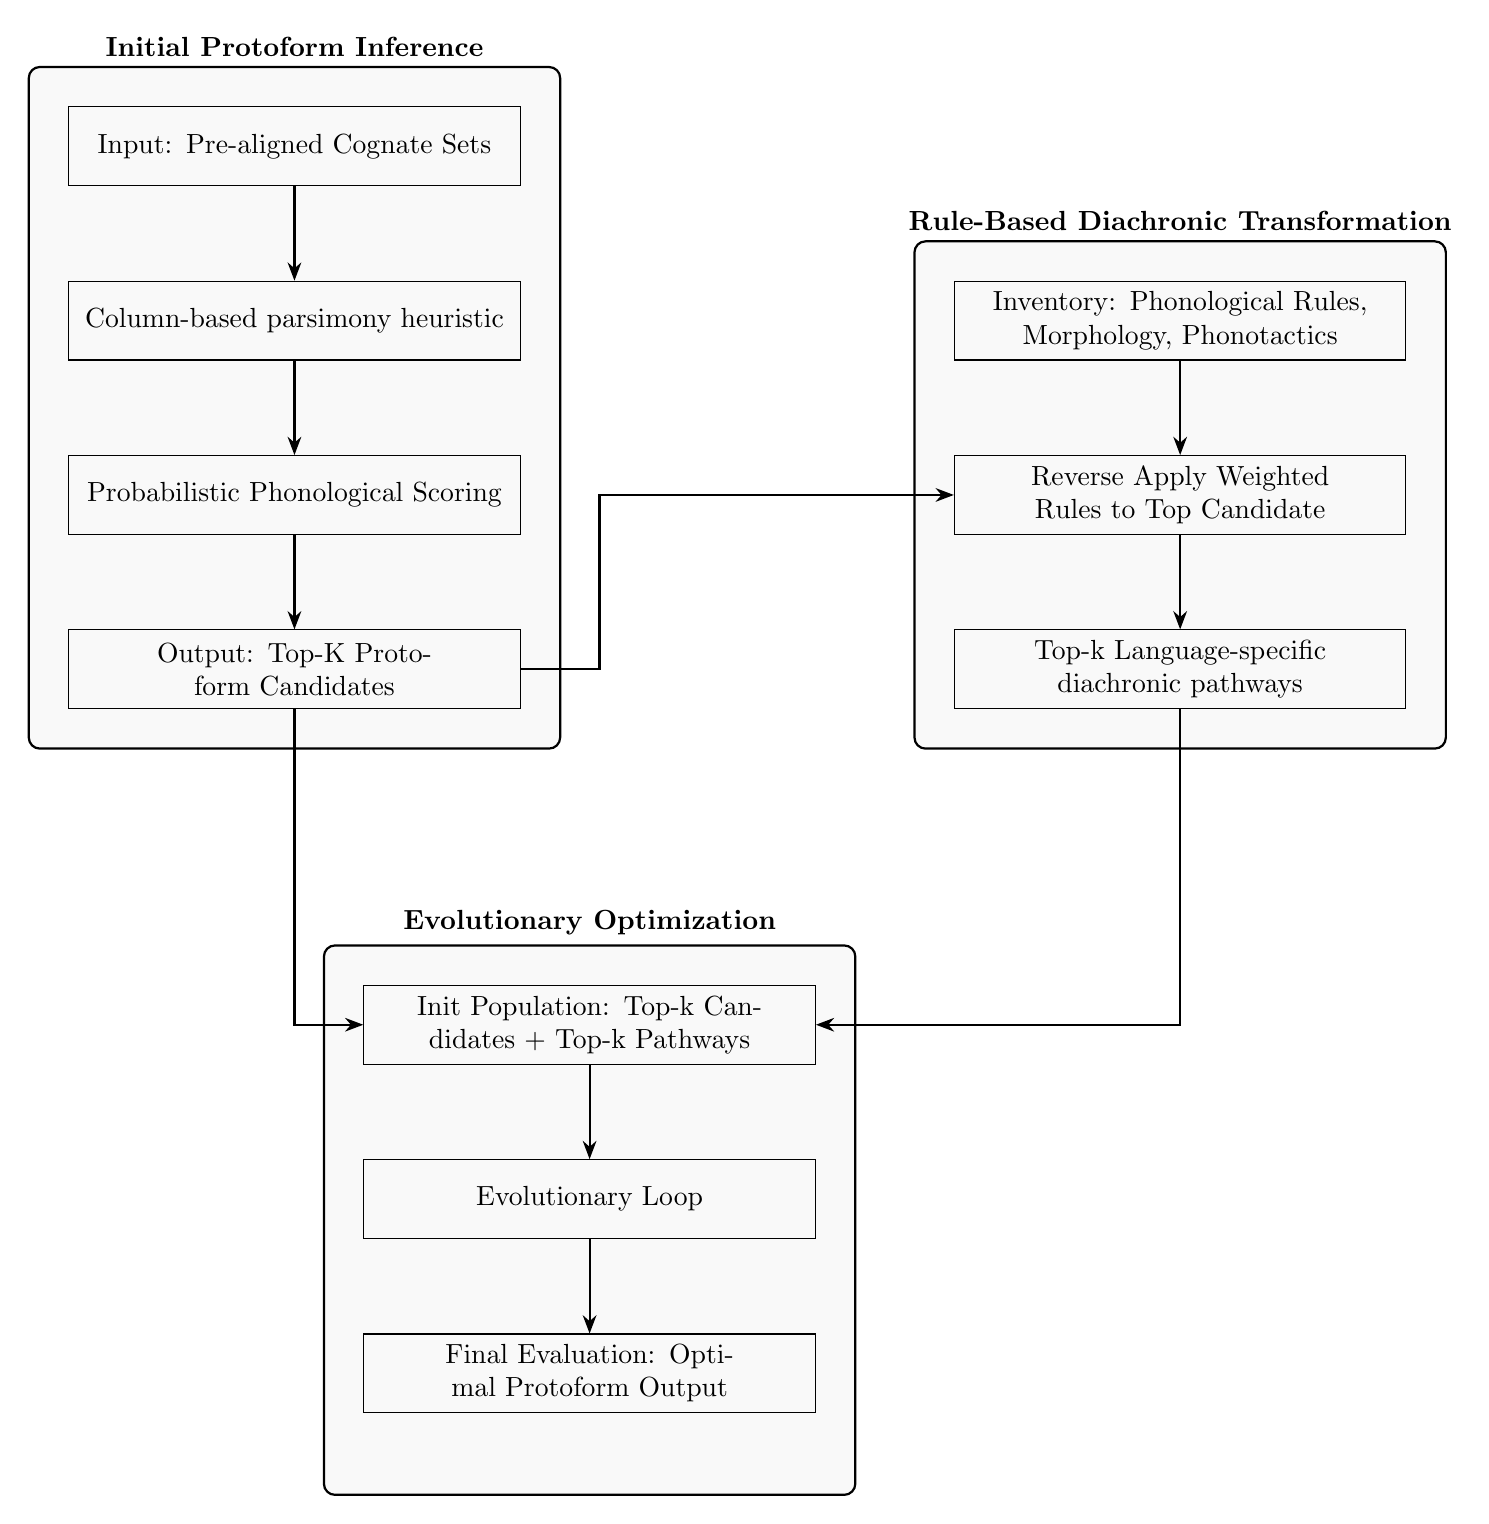
\begin{tikzpicture}[
  node distance=1.2cm and 2.5cm,
  phasebox/.style={draw, rounded corners, thick, inner sep=0.5cm, fill=gray!5},
  mystep/.style={rectangle, draw, minimum height=1cm, text width=5.5cm, text centered},
  arrow/.style={-Stealth, thick}
]

% Phase I nodes
\node[mystep] (align) {Input: Pre-aligned Cognate Sets};
\node[mystep, below=of align] (beamsearch) {Column-based parsimony heuristic};
\node[mystep, below=of beamsearch] (probscore) {Probabilistic Phonological Scoring};
\node[mystep, below=of probscore] (protoforms) {Output: Top-K Protoform Candidates};

% Phase I box
\begin{pgfonlayer}{background}
\node[phasebox, fit=(align)(beamsearch)(probscore)(protoforms), label=above:{\textbf{Initial Protoform Inference}}] (phase1) {};
\end{pgfonlayer}

% Phase II nodes
\node[mystep, right=5.5cm of beamsearch] (rules) {Inventory: Phonological Rules, Morphology, Phonotactics};
\node[mystep, below=of rules] (revapply) {Reverse Apply Weighted Rules to Top Candidate};
\node[mystep, below=of revapply] (rankedreflexes) {Top-k Language-specific diachronic pathways};

% Phase II box
\begin{pgfonlayer}{background}
\node[phasebox, fit=(rules)(revapply)(rankedreflexes), label=above:{\textbf{Rule-Based Diachronic Transformation}}] (phase2) {};
\end{pgfonlayer}

% Phase III nodes
\node[mystep, below right=3.5cm and -2cm of protoforms] (evoinit) {Init Population: Top-k Candidates + Top-k Pathways};
\node[mystep, below=of evoinit] (evoloop) {
  Evolutionary Loop
};
\node[mystep, below=of evoloop] (finaleval) {Final Evaluation: Optimal Protoform Output};

% Add padding below the last node
\node[below=0.5cm of finaleval, inner sep=0pt, outer sep=0pt] (padding) {};

% Phase III box
\begin{pgfonlayer}{background}
\node[phasebox, fit=(evoinit)(evoloop)(finaleval)(padding), label=above:{\textbf{Evolutionary Optimization}}] (phase3) {};
\end{pgfonlayer}

% Arrows between phases
\draw[arrow] (align) -- (beamsearch);
\draw[arrow] (beamsearch) -- (probscore);
\draw[arrow] (probscore) -- (protoforms);
\draw[arrow] (protoforms.east) -- ++(1,0) |- (revapply.west);
\draw[arrow] (rules) -- (revapply);
\draw[arrow] (revapply) -- (rankedreflexes);
\draw[arrow] (protoforms.south) -- ++(0,-0.6) |- (evoinit.west);
\draw[arrow] (rankedreflexes.south) -- ++(0,-0.6) |- (evoinit.east);
\draw[arrow] (evoinit) -- (evoloop);
\draw[arrow] (evoloop) -- (finaleval);

\end{tikzpicture}
\end{document}